% Presetting

    \documentclass[11pt]{book}

    \RequirePackage{silence}
    \WarningFilter{remreset}{The remreset package}

    % Chapter Style

            % Headings  
            \usepackage[Glenn]{fncychap}
            \ChNumVar{\fontsize{40}{42}}
            \ChTitleVar{\Large\sc}
            \ChNameVar{\empty}
            \setlength\headheight{14.5pt}
            
            % Roman Numerals
            \usepackage{remreset}
            \renewcommand*\thechapter{\Roman{chapter}}
            \renewcommand*\thesection{\arabic{section}}
            \makeatletter
            \@removefromreset{section}{chapter}
            \makeatother

            % Head Style
            \renewcommand\FmN[1]{\Large \sc Partie}

    % Mathematics

            % Formatting
            \usepackage{amsmath}
            \usepackage{amsfonts,amssymb}
            \usepackage{tasks,environ}
            \usepackage{xargs}
                
            %Custom Shortcuts
            \newcommand{\eqi}{\Leftrightarrow}
            \newcommand{\lr}[1]{\left( #1 \right)}
            \newcommand{\limit}[1]{\displaystyle{\lim_{#1}}}
            \newcommand{\tab}{\hspace*{7mm}}
            \newcommand{\ds}[1]{\displaystyle{#1}}
            \newcommand{\floor}[1]{\lfloor #1 \rfloor}
            \newcommand{\R}{\mathbb{R}}
            \newcommand{\seg}[1]{\overline{\rm {#1}}}
            \newcommand{\Int}{\int\limits}
            \newcommand{\ex}{\tab \uline{Example :}\hspace{0.2cm} }
            \newcommand{\note}{\tab \uline{Note :}\hspace{0.2cm} }
            \newcommand{\vard}{\partial}
            \newcommand{\Q}{\mathcal{Q}}
            \renewcommand{\Re}{\operatorname{Re}}
            \renewcommand{\Im}{\operatorname{Im}}
            \renewcommand{\P}{\mathcal{P}}
            \newcommand{\tc}[2]{\textcolor{#1}{#2}}

            
            % Colors
            \usepackage{xcolor}
            \newcommand{\blu}{\color{blue}}
            \newcommand{\Red}{\color{red}}
            \newcommand{\blac}{\color{black}}
            
            \newcommand{\red}[1]{\textcolor{red}{#1}}

            \definecolor{blue}{RGB}{0,224,224}
            \definecolor{yellow}{RGB}{221,221,0}
            
        \usepackage{xcolor,xspace}
        \usepackage{amssymb}
        
    % Page Style
            
            % Cover Page 
            \usepackage{tikz}
            \makeatletter
            \def\parsecomma#1,#2\endparsecomma{\def\page@x{#1}\def\page@y{#2}}
            \tikzdeclarecoordinatesystem{page}{
                \parsecomma#1\endparsecomma
                \pgfpointanchor{current page}{north east}
                % Save the upper right corner
                \pgf@xc=\pgf@x%
                \pgf@yc=\pgf@y%
                % save the lower left corner
                \pgfpointanchor{current page}{south west}
                \pgf@xb=\pgf@x%
                \pgf@yb=\pgf@y%
                % Transform to the correct placement
                \pgfmathparse{(\pgf@xc-\pgf@xb)/2.*\page@x+(\pgf@xc+\pgf@xb)/2.}
                \expandafter\pgf@x\expandafter=\pgfmathresult pt
                \pgfmathparse{(\pgf@yc-\pgf@yb)/2.*\page@y+(\pgf@yc+\pgf@yb)/2.}
                \expandafter\pgf@y\expandafter=\pgfmathresult pt
            }
            \makeatother
            
            
            % Object formatting
            \usepackage[12pt]{moresize}
            \usepackage{titlesec}
            \usepackage{import}
            \usepackage{floatrow}
            \usepackage{enumitem}
            \usepackage{changepage}
            \usepackage[normalem]{ulem}
            
            \usepackage{caption}
            \DeclareCaptionFormat{underline}{\uline{#1}#2#3\par}
            \captionsetup[figure]{labelformat=empty}
            
            \titleformat{\section}{\Large \bfseries \filcenter}{\uline{Section \thesection}}{1em}{\uline}

            \usepackage{makecell}
            \renewcommand\theadalign{bc}
            \renewcommand\theadfont{\bfseries}
            \renewcommand\theadgape{\Gape[4pt]}
            \renewcommand\cellgape{\Gape[4pt]}
            
            % Geometry
            \usepackage{fancyhdr}
            \usepackage{ragged2e}
            \usepackage[a4paper, total={18.625cm, 22.125cm}]{geometry}
            
            % Typewritting

            \setlength{\parskip}{1em}
            \setlength{\parindent}{0em}
            \newcommand{\ul}{\underline}

            % Header & Footers
            \renewcommand{\chaptermark}[1]{\markboth{#1}{#1}}
            \renewcommand{\sectionmark}[1]{
                \markright{ #1}
            }
            \pagestyle{fancy}
            \fancyhf{}
            \fancyhead[RE, LO]{\text{\rightmark}}
            \fancyfoot[LE, RO]{\textbf{Page \thepage}}
            
            
            \fancypagestyle{plain}{%
            \fancyhf{} % clear all header and footer fields
            \fancyfoot[LE, RO]{\textbf{Page \thepage}}
            \renewcommand{\headrulewidth}{0pt}
            \renewcommand{\footrulewidth}{0pt}}
            
            % List Formatting
            \NewEnviron{items}[3][0pt]{
              \vspace{#2}
              \begin{itemize}
                \setlength{\itemsep}{#1}
                \setlength{\topsep}{0pt}
                \setlength{\partopsep}{0pt}
                    \BODY
              \end{itemize}\vspace{#3}}
            
            \NewEnviron{enum}[3][0pt]{%
              \vspace{#2}%
              \begin{enumerate}%
                \setlength{\itemsep}{#1}%
                \setlength{\topsep}{0pt}%
                \setlength{\partopsep}{0pt}%
                    \BODY
              \end{enumerate}
              \vspace{#3}}%
              
            \NewEnviron{eq}[2]{%
              \vspace{#1}%
              \begin{align*}%
                    \BODY
              \end{align*}
              \vspace{#2}}%
            
            \NewEnviron{dent}[1]{
                \begin{adjustwidth}{7mm}{}
                \uline{#1}\hspace{2mm} 
                    \BODY
                \end{adjustwidth}
            }
            \NewEnviron{lfeq}[2]{%
              \vspace{#1}%
              \begin{flalign*}%
                    \BODY
              \end{flalign*}
              \vspace{#2}}%
                 
    % Table of Contents

        \usepackage{titletoc}
        \usepackage{erewhon, cabin}    
        \usepackage{hyperref}
        \renewcommand*\contentsname{\centerline{Table des Contenus}}

        \setcounter{secnumdepth}{0}
        \setcounter{tocdepth}{2}
        
        \usepackage{tocloft}
        \setlength\cftparskip{0pt}
        
        \usepackage{etoolbox}
        \makeatletter
        \pretocmd{\chapter}{\addtocontents{toc}{\protect\addvspace{5\p@}}}{}{}
        \pretocmd{\section}{\addtocontents{toc}{\protect\addvspace{-10\p@}}}{}{}
        \pretocmd{\subsection}{\addtocontents{toc}{\protect\addvspace{-10\p@}}}{}{}
        \makeatother
        
            % Chapter Style
            \titlecontents{chapter}
                [11em] %5.3
                {\bigskip}
                {\contentslabel[\bfseries\textsc{Partie \thechapter}~\thecontentslabel]{6em}\textbf}%\thecontentslabel
                {\hspace*{-5.5em}\textbf}% unnumbered chapters
                {\titlerule*[1pc]{ }}[\smallskip]
                
            % Section Style
            \titlecontents{section}
            [5.5em] % i
            {\bigskip\bigskip}
            {\large\thecontentslabel\enspace\textbf}%\thecontentslabel
            {\hspace*{-5.5em}\textbf}
            {\titlerule*[1pc]{.}\contentspage}

            % Subsection Style
            \titlecontents{subsection}
            [8.5em] % i
            {\bigskip}
            {\thecontentslabel\enspace\textbf}%\thecontentslabel
            {\hspace*{-5.5em}\textbf}
            {\titlerule*[1pc]{}}
                
    % Functions and Data Plotting
        \usepackage{subfig,wrapfig,adjustbox,multirow}
            
            % Circuit Drawing
            \usepackage[american]{circuitikz} 
            \usetikzlibrary{decorations.pathreplacing,decorations.pathmorphing,calligraphy}
            
            % Plotting Style
            \usepackage{graphicx,pgfplots}
            \usetikzlibrary{arrows.meta}
            \usetikzlibrary {patterns,patterns.meta}
            \usepgfplotslibrary{fillbetween}
            \pgfplotsset{compat=1.18}


            
            \usepgfplotslibrary{units}
            % Logarithmic Scale
            \pgfplotsset{
                log x ticks with fixed point/.style={
                    xticklabel={
                        \pgfkeys{/pgf/fpu=true}
                        \pgfmathparse{exp(\tick)}%
                        \pgfmathprintnumber[fixed relative, precision=3]{\pgfmathresult}
                        \pgfkeys{/pgf/fpu=false}
                    }
                }
            }

\begin{document}

% Page settings

    % Section Spacing
        \titlespacing\section{0pt}{3pt plus 2pt minus 2pt}{6pt plus 2pt minus 1pt}
        \titlespacing\subsection{0pt}{0pt plus 2pt minus 2pt}{0pt plus 4pt minus 2pt}

    % Cover
        \begin{titlepage}
            \newgeometry{top=1cm, width=21cm, bottom=1cm}           
            
            \begin{tikzpicture}[remember picture,overlay,every node/.style={anchor=center}]


                \node[opacity =0.07, inner sep=0pt, anchor=east] at (current page.east){\includegraphics[width=0.5\paperwidth,height=\paperheight]{./logos/invert1.jpg}};

                \node[opacity=0.15, inner sep=0pt, anchor=south west] at (current page.south west){\includegraphics[width=0.5\paperwidth,height=0.5\paperheight]{./logos/invert2.jpg}};

                \node[opacity=0.15,inner sep=0pt, anchor=north west] at (current page.north west){\includegraphics[width=0.5\paperwidth,height=0.5\paperheight]{./logos/invert3.jpg}};

                \node at (page cs:0,0.9) {\includegraphics[height=1cm]{./logos/IMT.png}\hspace{1.5cm}\includegraphics[height=1.5cm]{./logos/UJM.png}};

                \node at (page cs:0,0.8) {\Large\textsc{Cycle Initial en Technologies de l'Information de Saint-Étienne}};

                \node at (page cs:0,0.5) {\HUGE\textbf{OSCILLATEURS}};
                \draw (page cs:0.5,0.45) -- (page cs:-0.5,0.45); 

                \node at (page cs:0,0.4) {\Large\textsc{Eva Maturana - Lucas Lescure}}; 

                \node[opacity=0.5] at (page cs:-0.7,-0.8) {\includegraphics[width=1.2\textwidth]{./logos/Logo-t.png}};

            \end{tikzpicture}          
        \end{titlepage}


    \newgeometry{width=18.625cm, bottom=2cm, top=2cm}

    \tikz[remember picture, overlay] \node[opacity=0.3,inner sep=0pt, anchor=north east] at (current page.north east){\includegraphics[angle=-90,origin=c,width=0.5\paperheight,height=0.5\paperwidth]{./logos/invert3.jpg}};
    \tikz[remember picture,overlay] \node[opacity=0.3,inner sep=0pt, anchor=south east] at (current page.south east){\includegraphics[angle=90,width=0.5\paperwidth,height=0.5\paperheight]{./logos/invert2.jpg}};

    \tableofcontents


    \newpage

\section{Oscillateur Pont de Wien}

    \subsection{Oscillateur}

        \begin{figure}[ht]
            \begin{floatrow}
                \ffigbox{\includegraphics[width=0.4\textwidth]{./object/c1.png}\caption{\ul{Circuit Oscillateur}}}

                \ffigbox{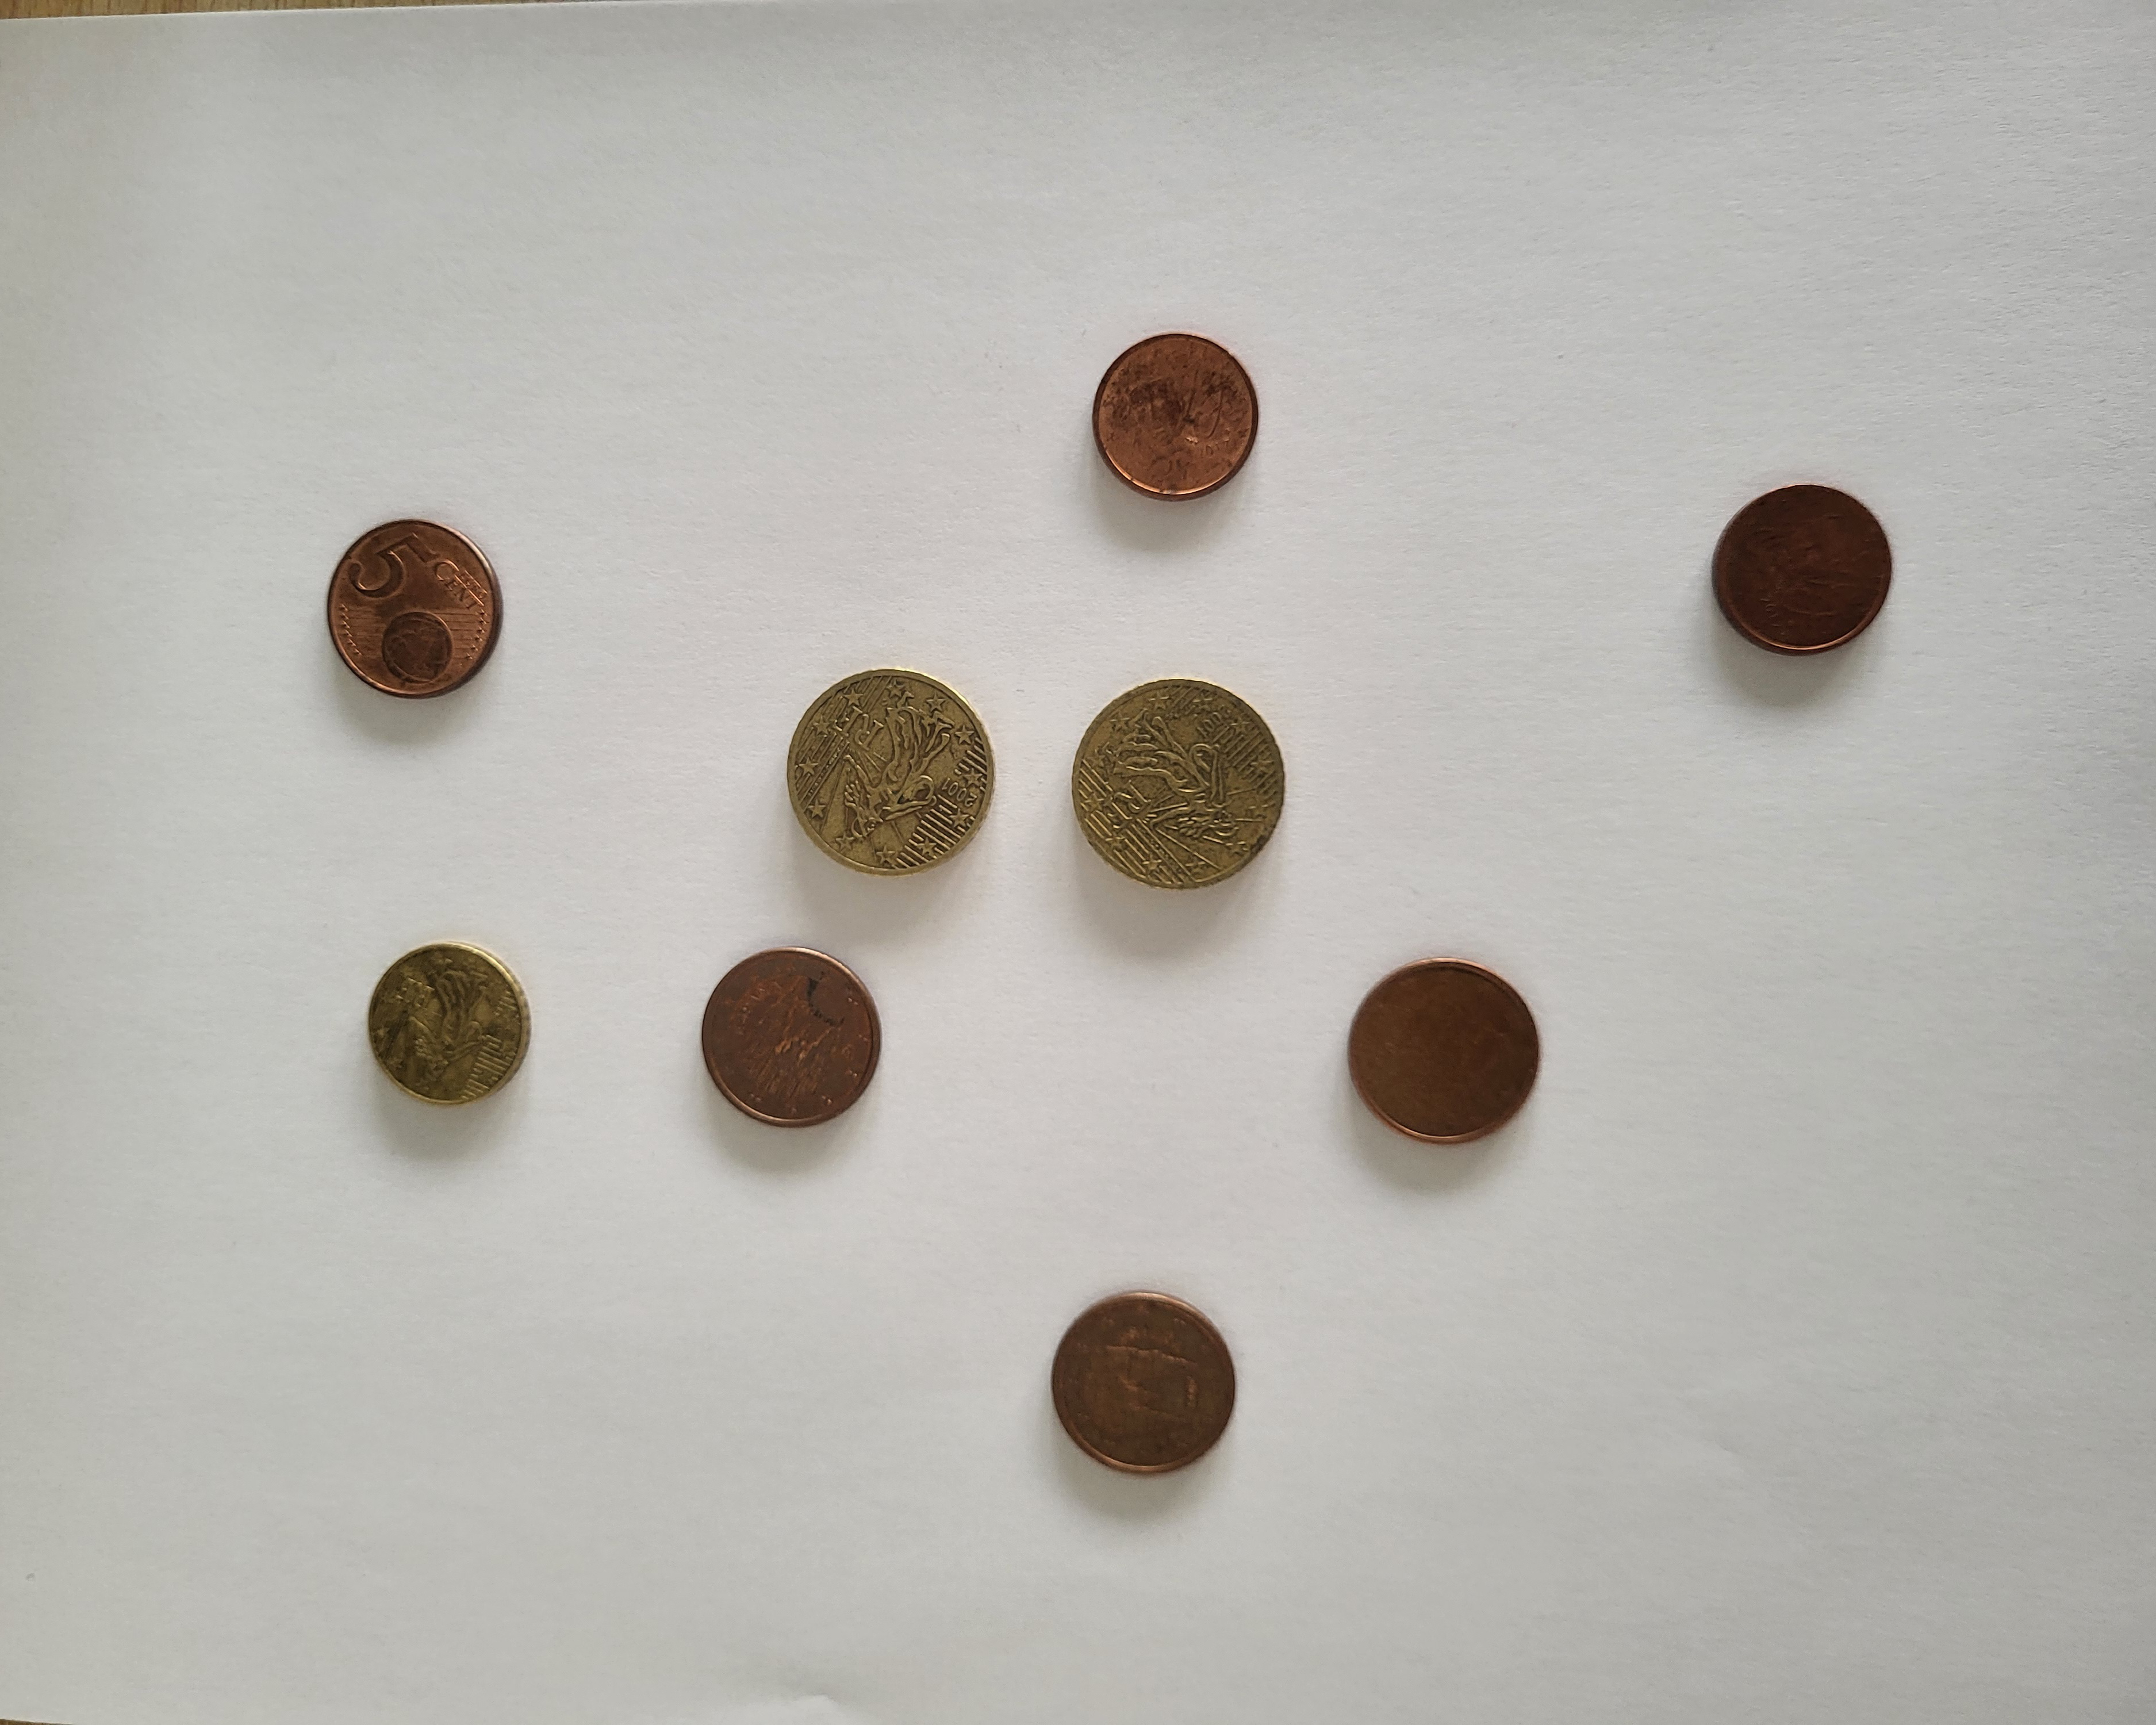
\includegraphics[width=0.4\textwidth]{./object/g1.png}\caption{\ul{Relevées de \textcolor{yellow}{$V_{C2}$} et \textcolor{blue}{$V_S$}}}}

            \end{floatrow}
        \end{figure}

        On voit que le circuit oscille autour de la fréquence théorique à $157\ H_z$. On constate une amplification $A=\frac{15.6}{5.12}=3$ ce qui resulte par un gain de $G=10\log{(3)}=4.77\ dB$.

        On retrouve une oscilation normale en sortie, pour ce faire il faut être vigilant sur le réglage de $P$.

    \subsection{Oscillateur avec stabilisation}

        \begin{figure}[ht]
                \includegraphics[width=0.4\textwidth]{./object/c2.png}
                \caption{\ul{Circuit Oscillateur avec Diodes}}
        \end{figure}

        \begin{figure}[ht]
            \begin{floatrow}
                \ffigbox{\includegraphics[width=0.4\textwidth]{./object/g2.png}\caption{\ul{\tc{blue}{$V_S$} et \tc{yellow}{$V_{C2}$} avec $P=100\Omega$}}}

                \ffigbox{\includegraphics[width=0.4\textwidth]{./object/g3.png}\caption{\ul{\tc{blue}{$V_S$} et \tc{yellow}{$V_{C2}$} avec $P=0\Omega$}}}

            \end{floatrow}
        \end{figure}

        On voit qu'en modifiant $P$ on arrive pas à avoir un signal qui soit parfaitement sinusoidal. La résistance dynamique des diode fait en sorte qu'on ai une sorte de rampe lorsque \tc{blue}{$V_S$} se rapproche de $0$. 

        \newpage

        Pour négliger cette resistance dynamique on rajoute donc une resistance de $1\ k\Omega$ en parallèle avec les diodes. Comme nous le voyons ci-dessous le signal est bien plus propre. 

        \begin{figure}[ht]
            \begin{floatrow}
                \ffigbox{\includegraphics[width=0.4\textwidth]{./object/g5.png}\caption{\ul{\tc{blue}{$V_S$} et \tc{yellow}{$V_{C2}$} avec $P=100\Omega$ et la resistance en parallèle}}}

                \ffigbox{\includegraphics[width=0.4\textwidth]{./object/g4.png}\caption{\ul{\tc{blue}{$V_S$} et \tc{yellow}{$V_{C2}$} avec $P=0\Omega$ et la resistance en parallèle}}}

            \end{floatrow}
        \end{figure}

        On voit donc qu'avec cette resistance l'socillation est plus propre, mais on perd aussi un peut en amplitude. 

\newpage

\section{Oscillateurs Collpit}

            Après avoir réglé le point de fonctionnement du transistor on calcule la fréquence d'oscillation suivante:\\

            \centerline{$\ds{\omega_0=\frac{1}{2\pi \sqrt{\frac{C_1C_2}{C_1+C_2}L}}=299\ kH_z}$}

        \subsection{Simulation Proteus}

            \begin{figure}[ht]
                \begin{floatrow}
                    \ffigbox{\includegraphics[width=0.4\textwidth]{./object/c4.png}\caption{\ul{Circuit du Collpit}}}

                    \ffigbox{\includegraphics[width=0.4\textwidth]{./object/prot.png}\caption{\ul{Diagramme de Bode}}}

                \end{floatrow}
            \end{figure}

            Pour que le montage puisse osciller on voit donc qu'il faut une fréquence à $300\ kH_z$ ce qui correspond à la valeur théorique. On peut aussi déduire que ce filtre est du $3^{eme}$ ordre puisque la pente est à $-60\ dB.dec^{-1}$ et la phase se situe sur un intervale de $270^{\circ}$.

    \subsection{Manipulation}
        
        \begin{figure}[ht]
            \centering
            \includegraphics[width=0.5\textwidth]{./object/g7.png}
            \caption{\ul{Réponse indicielle, \tc{blue}{$V_1$} et \tc{yellow}{$V_2$}}}
        \end{figure}

        En cablant le montage on relève une même fréquence d'oscillation à $300\ kH_z$. On peut aussi determiner que ce filtre est inverseur car le signal est déphasé de $180^{\circ}$.

        Pour $470\ pF$ on relève par simulation une fréquence d'oscillation à environ $1\ MH_z$

        \newpage

        \begin{figure}[ht]
            \centering
            \includegraphics[width=0.5\textwidth]{./object/g8.png}
            \caption{\ul{Réponse indicielle, \tc{blue}{$V_1$} et \tc{yellow}{$V_2$}}}
        \end{figure}

        En cablant ce montage sur la maquette on obtient une fréquence d'oscillation à $745\ kH_z$. Ceci est dû à la capacitée parasite des cables coaxiaux qui modifient donc la capacitance du circuit et ainsi modifient la fréquence d'oscillation.



    \subsection{Etude I de l'influence des cables BNC}

        En débranchant $V_2$ on obtient la réponse suivante:

        \begin{figure}[ht]
            \begin{floatrow}
                \ffigbox{\includegraphics[width=0.4\textwidth]{./object/c5.png}\caption{\ul{Circuit de l'oscillateur}}}

                \ffigbox{\includegraphics[width=0.4\textwidth]{./object/g9.png}\caption{\ul{Réponse Indicielle}}}

            \end{floatrow}
        \end{figure}

        On obtient une fréquence de $800\ kH_z$ ce qui se rapproche de la simulation éfféctuée précédemment.

        Faisant de même en échangeant $V_1$ et $V_2$ on obtient:

        \begin{figure}[ht]
            \begin{floatrow}
                \ffigbox{\includegraphics[width=0.4\textwidth]{./object/c6.png}\caption{\ul{Circuit de l'oscillateur}}}

                \ffigbox{\includegraphics[width=0.4\textwidth]{./object/g10.png}\caption{\ul{Réponse Indicielle}}}

            \end{floatrow}
        \end{figure}

        La fréquence d'oscillation est à $750\ kH_z$, ce qui est toujours moins que la simulation, mais aussi ne change pas grand chose par rapport au circuit avec $V_1$ et $V_2$ de branchées.

    \subsection{Etude II de l'influence des cables BNC}
        On supprimme maintenant les deux capacitor de $470\ pF$, et on rebranche $V_1$ et $V_2$ :

        \begin{figure}[ht]
            \begin{floatrow}
                \ffigbox{\includegraphics[width=0.4\textwidth]{./object/c7.png}\caption{\ul{Circuit de l'oscillateur}}}

                \ffigbox{\includegraphics[width=0.4\textwidth]{./object/g11.png}\caption{\ul{Réponse Indicielle}}}

            \end{floatrow}
        \end{figure}

        Cette fois-ci la fréquence d'oscillation est à $1.5\ MH_z$ ce qui est bien supérieur aux deux circuits précédent mais dépasse la fréquence trouvée en simulation.

        On débranche $V_2$ encore une fois, laissant $V_1$ :

        \begin{figure}[ht]
            \begin{floatrow}
                \ffigbox{\includegraphics[width=0.4\textwidth]{./object/c8.png}\caption{\ul{Circuit de l'oscillateur}}}

                \ffigbox{\includegraphics[width=0.4\textwidth]{./object/g12.png}\caption{\ul{Réponse Indicielle}}}

            \end{floatrow}
        \end{figure}

        La fréquence d'oscillation est à $4.2\ MH_z$

        On débranche $V_1$ et rebranche $V_2$ : 

        \begin{figure}[ht]
            \begin{floatrow}
                \ffigbox{\includegraphics[width=0.4\textwidth]{./object/c9.png}\caption{\ul{Circuit de l'oscillateur}}}

                \ffigbox{\includegraphics[width=0.4\textwidth]{./object/g13.png}\caption{\ul{Réponse Indicielle}}}

            \end{floatrow}
        \end{figure}

        La fréquence d'oscillation est à $2.16\ MH_z$. 


        On en conclut que pour pour ce type d'oscillateur, l'utilisation de faibles capacitances pour augmenter la fréquence d'oscillation est une mauvaise idée. Lorsqu'elle sont très faibles les capacitances parasites, qui peuvent provenir de l'environment ou du circuit, s'ajoutent à celles qui sont déjà présentes, et modifie donc la fréquence de l'oscillation de façon indésirable.\\
        Pour éviter cet effet il faut donc utiliser des capacitance un peu plus fortes de façon à pouvoir négliger ces parasites et controller la fréquence d'oscillation. 

\newpage

\section{Oscillateur Clapp}
    
    Avec l'oscillateur Clapp si l'on veut une fréquence de $900\ kH_z$ avec $C_1=2.2\ nF$ et $C_2=1.5\ nF$ on applique la formule ci-dessous (dérivée des formules du TP): 

    \centerline{$\ds{C_3=\frac{1}{L(2\pi f)^2-(\frac{1}{C_1}+\frac{1}{C_2})}}$}

    Ainsi on obtient $C_3=370\ pF$. La capacitance la plus proche normalisée est donc celle à $470\ pF$.

    On relève la réponse indicielle suivante:

    \begin{figure}[ht]
        \begin{floatrow}
            \ffigbox{\includegraphics[width=0.4\textwidth]{./object/c10.png}\caption{\ul{Circuit de l'oscillateur}}}

            \ffigbox{\includegraphics[width=0.4\textwidth]{./object/g14.png}\caption{\ul{Réponse Indicielle}}}

        \end{floatrow}
    \end{figure}

    La fréquence de l'oscillation est à $780\ kH_z$ ce qui est moins que les $828\ kH_z$ attendu, mais qui s'explique par le fait que l'on utilise pas une capacitances faibles, et donc prônes à subir les effets des capacitances parasites du  cable BNC.  

    On observe une atténuation de $0.99$ ce qui est proche de la valeur théorique $\frac{C_1}{C_2+C_3}=1.1$, et qui peut s'expliquer par les parasites des cables BNC. 

\end{document}